\section{Лирика}
\subsection{Общие сведения}
Расширение сфер применения компьютерной техники обусловлено ростом производительности и информационной емкости вычислительных систем, 
что в свою очередь зависит от успехов в развитии аппаратуры и программного обеспечения(ПО). 
А успехи в развитии аппаратуры определяются сегодня в первую очередь степенью интеграции элементной базы, 
развитием технологий обработки информации, развитием коллективного использования сетевых распределенных ресурсов. 
Успехи в развитии ПО требуют использования всех средств автоматизации программирования для получения максимальной эффективности, скорости выполнения критических участков программ. 
Для решения этой задачи большую роль играет использование машинно-ориентированных языков.

Выделяют две основные сферы применения машинно зависимых языков:
\begin{itemize}
    \item создание системных программ, входящих в состав драйверов нестандартных машинных устройств
    \item решение специфических задач для информационных и управляющих систем, например систем реального времени.
\end{itemize}

При классификации программных средств, традиционно их делят на
\begin{itemize}
    \item Прикладные (пользовательские), ориентированные на конечного пользователя
    \item Системные, поддерживающие работу вычислительной системы в автоматическом режиме
\end{itemize}
Прикладные программы включают в себя пакеты прикладных программ, библиотеки объектных модулей
которые используются для решения задач, в конкретной области применения техники.
К классу системных программ, относятся программы, которые обеспечивают автоматический режим работы вычислительной системы
а также разработку, модификацию различных программ, как прикладных, так и системных.

Управляющие системные программы, обеспечивающие корректное выполнение всех процессов
при решении задач и функционировании системы постоянно сохраняются в оперативной памяти,
составляют ядро операционной системы и называются резидентными.
Управляющие программы, которые подргужаются в оперативную память по мере необходимости, перед их выполнением
называются транзитными. 

Обрабатывающие системные программы выполняются, как специальные проблемные или приложения операционных систем
используемых при разработке новых и модификации уже разработанных программ.

\subsection{Почему ассемблер?}

Разработка системных программ, требует использование специальных системных языков программирования, это могут быть машинно-зависимые языки "--- <<ассемблеры>> или такие языки как С или PLM, а также языки
высокого уровня, которые имеют развитые средства работы с внутренней адресной информацией.

Язык Ассемблер используется везде, где необходима максимальная производительность и эффективность, 
ет использоваться до тех пор, пока проводятся исследовательские работы в области 
развития и создания новых архитектур ЭВМ. 

Кроме того, многие языки высокого уровня имеют возможность использования ассемблерных 
вставок, поэтому говорят, что языки ассемблера и языки низкого уровня сохраняют свое значение, в областях, 
где требуется высокая скорость выполнения кода,
и будут использоваться до тех пор, пока идет процесс совершенстования архитектур процессоров.

Сферы применения языка:
\begin{enumerate}
    \item все, что требует максимальной скорости выполнения (основные компоненты компьютерных игр, ядра ОС реального времени).
    \item все, что непосредственно взаимодействует с внешними устройствами.
    \item все, что полностью использует возможности процессора (ядра многозадачных ОС, программы перевода в защитный режим).
\end{enumerate}

К недостаткам языка принято относить сложность в изучении, плохую читаемость, непереносимость на другие процессоры.

\section{Архитектура ПК}
Архитектура ПК включает в себя структурную организацию, т.е организацию аппартных средств, 
наличие блоков устройств, а также функциональную организацию
позволяющую организовать программное управление этой вычислительной системы. 
С точки зрения программиста, архитектура ПК это совокупность программно доступных средств.

\begin{figure}[H]
    \centering
    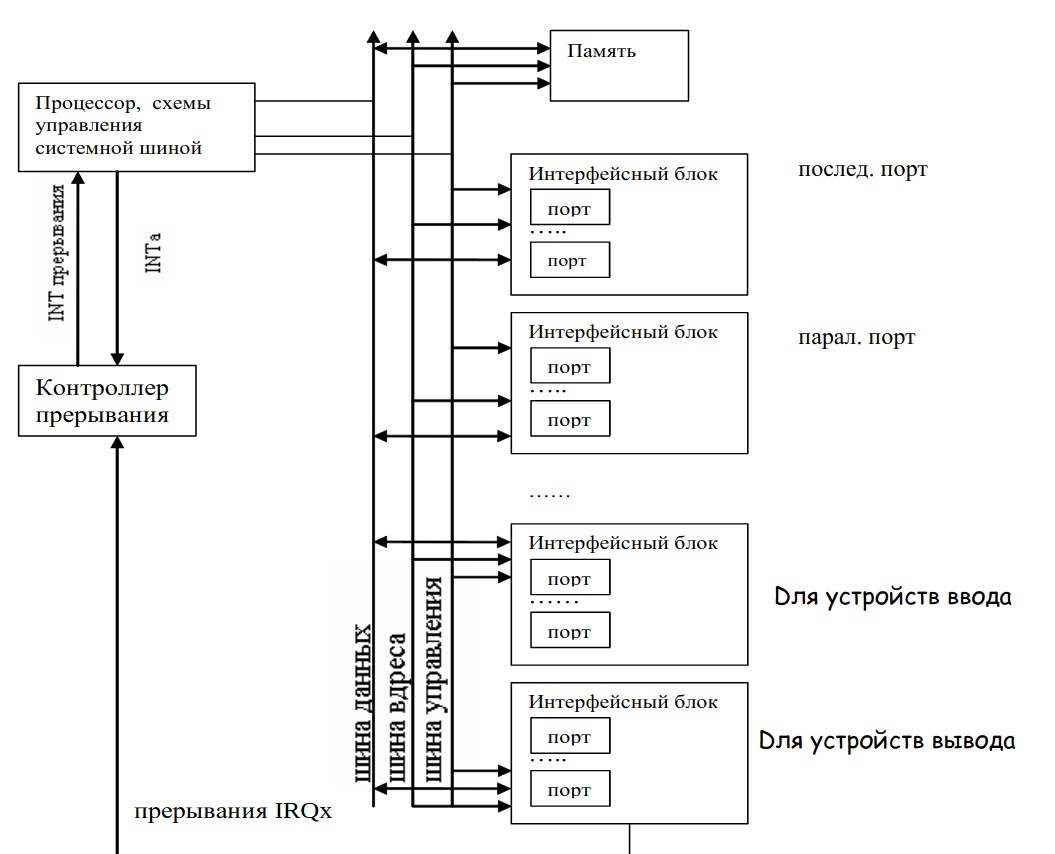
\includegraphics[scale = 0.4]{structurePC.jpg}
\end{figure}

Она строится на магистрально"=модульном принципе, который заключается в том что к системной шине в центральной магистрали стандартным образом, 
с помощью стандартного интерфейса подключаются все устройства.
Системная шина включает в себя шину данных, адресную шину и шину управления.
Шины "--- это набор линий связи, по которым информация передается от одного из участников к одному или нескольким приемникам.

Внешние устройства работают значительно медленне ЦП, поэтому в архитектуру ПК подключен, не отраженный на схеме канал прямого доступа к памяти, 
а для связи с внешними устройствами используется интерфейсные блоки, представляющие собой устройства управления внешними устройствами.
который содержит в себе собственные шины данных, шины управления, адресную шину.

Канал прямого доступа к памяти и интерфейсные блоки, позволяют обеспечить параллельную работу процессора и внешних устройств
но для синхронизации действий всех устройств используется система прерываний.
Он может быть как один, так и каскадный контроллер, в зависимости от количества подключенных внешних устройств.

Организация работы вычислительной системы может осуществляться следующим образом "---
когда какому либо устройству требуется работа процессора, например, ввести данные или вывести
это устройство посылает процессору специальный сигнал прерывания, он проходит через контроллер прерываний, если процессор может обслужить прерывание
этот сигнал передается процессору.Процессор его изучает и возвращает его с именем int a затем формируется номер прерывания, процессор прерывает выполнение текущей программы,
запомнив предварительно следующую команду, которая должна была выполнятся и передает управление на выполнение программы обработки выполнения этого прерывания.

Если прерывание успешно обработано, то процессор продолжает выполнение прерванной программы.
прерывания бывают различные, это могут быть внешние/внутренние прерывания, системные, программные, маскированные/немаскированные
начальный адресат программ обработки прерываний хранятся в спец таблице вектора прерываний

\subsection{Архитектура микропроцессора ix86}

Процессор ix86 после включения питания устанавливается в реальныйрежим адресации памяти и работы процессора. 
Большинство ОС сразу переводит его в защищенный режим, обеспечивает многозадачность, распределение памяти, ресурсов и других дополнительных возможностей. 
Программы пользователей в таких ОС могут работать в еще одном режиме, 
режиме виртуальных машин, из которого доступно все, что доступно из реального режима и недоступны команды, относящиеся к защищенному режиму.

Совокупность программно-доступных средств процессора называется архитектурой процессора, с точки зрения программиста.
Начиная с i386 процессора программисту доступны 16 основных регистров, 11 регистров для работы с сопроцессором и мультимедийными приложениями, 
и в реальном режиме доступны некоторые регистры управления и некоторые специальные регистры.
Все команды, так или иначе, изменяют состояние регистров. Регистровая память является самой быстрой. 
Регистр "---- это набор из n устройств, способных хранить n"=разрядное двоичное число.
Схематично процессор можно представить в следующей виде:
\begin{figure}[H]
    \centering
    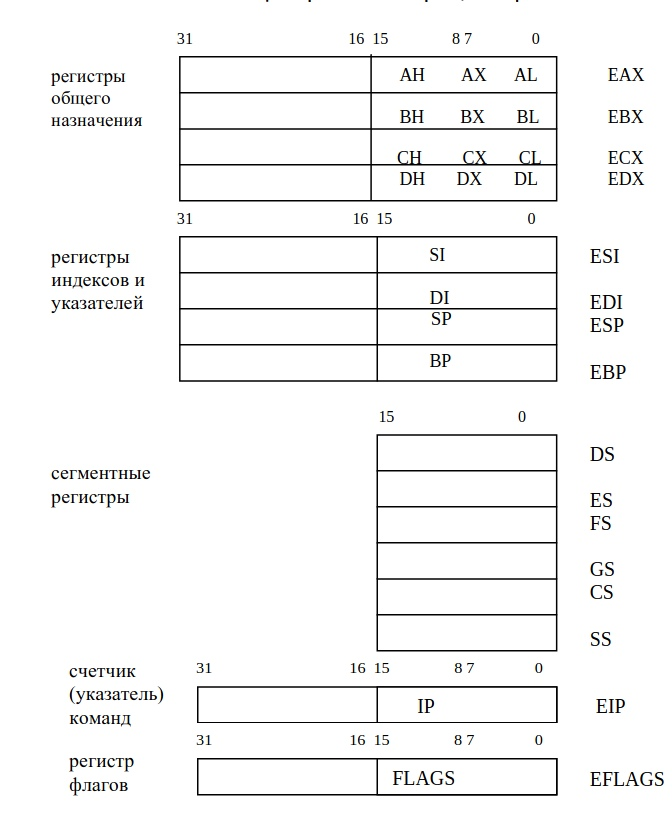
\includegraphics[scale = 0.5]{processor.jpeg}
\end{figure}

AX "--- аккумулятор, в нем хранится результат, если в один регистр не умещается, то старшая часть DX "--- регистр данных.
BX "--- используется для адресации по базе, CX "--- счетчик, используется в командах сдвига, регистры SP и BP используются при работе со стеком.

Регистры указателей и индексов имеют специальные назначения. Регистры индексов используются для организации способов адресации операндов, а регистры указателей "--- для организации работы с сегментом стека.

